\section{Historias de usuario}
\label{s:hu}
Las HU ser�n representadas mediante tablas divididas por las siguientes secciones:
\begin{description}

	\item [N�mero] Identificador entero incremental en el tiempo;
	\item [Nombre de historia de usuario] Identificador alfanum�rico para su uso
	      entre los desarrolladores y el cliente;
	\item[Usuario] Nombre y apellidos de la persona involucrada en el desarrollo de la \ac{hu};
	\item[Iteraci�n asignada] Identificador entero perteneciente a la iteraci�n en la cual se planea implementar la funcionalidad descrita en la \ac{hu};
	\item[Prioridad en negocio] Las historias de usuarios que describen funcionalidades imprescindibles en el desarrollo del sistema tienen prioridad alta; aquellas que debe tener el sistema, pero que no son necesarias para su funcionamiento, prioridad media; y auxiliares y que son independientes del sistema, prioridad baja.
	\item[Riesgo en desarrollo] Las historias de usuarios que, en caso de tener alg�n error de implementaci�n, puedan afectar la disponibilidad del sistema, tienen un riesgo de desarrollo alto; las \ac{hu} que puedan presentar errores y retrasan la entrega de la versi�n tienen riesgo de desarrollo medio; y las que puedan presentar errores, pero estos son tratados con facilidad y no afectan en desarrollo del proyecto, tienen riesgo de desarrollo bajo.

	\item[Puntos estimados] Tiempo estimado que tardar� el desarrollo de la \ac{hu};
	\item[Descripci�n] Breve descripci�n de \ac{hu};
	\item[Observaciones] Se�alamiento o advertencia del sistema;
	\item[Prototipo de interfaz] Prototipo de interfaz si aplica.
\end{description} \citep{Joskowicz2008}


Los t�tulos de las \ac{hu} generadas son:
\begin{enumerate}[label=HU \arabic*:]
	\item Autenticar usuario.
	\item Crear denuncia
	\item Actualizar denuncia
	\item Eliminar denuncia
	\item Crear resoluci�n
	\item Exportar resoluci�n.
\end{enumerate}
A continuaci�n se presentan algunas de las historias de usuarios identificadas en la investigaci�n
\begin{userstory}
	\storyname{Autenticar usuario}
	\storyuser{\authorA}
	\storyiter{1}
	\storypriority{ Alta }
	\storyrisk{ Bajo }
	\storypoints{0.6}
	\storyprogrammer{\authorA }
	\storydescription{El sistema debe permitir que los usuarios se autentiquen y tengan acceso s�lo a las funcionalidades correspondientes a su rol.}
	\storyobservation{}
	\storyinterface{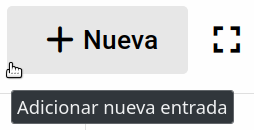
\includegraphics[scale=0.5]{images/prototypes/cdis-create-capture.png}}

\end{userstory}

\begin{userstory}
	\storyname{Crear denuncia}
	\storyuser{\authorA}
	\storyiter{1}
	\storypriority{ Alta }
	\storyrisk{ Bajo }
	\storypoints{1}
	\storyprogrammer{\authorA }
	\storydescription{El sistema debe permitir registrar una denuncia en el sistema. Para ello se le debe brindar al usuario un formulario en el que ingresar los datos de la nueva denuncia y botones para registrarla en el sistema o cancelar la acci�n.
		Los datos a ingresar en el formulario deben ser:
		\begin{itemize}
			\item Estudiantes involucrados
			\item Fecha de ocurrencia de los hechos descritos en la denuncia
			\item Hora de ocurrencia de los hechos descritos en la denuncia
			\item Descripci�n
			\item Adjuntos (\textit{opcional})
		\end{itemize}}
	\storyobservation{Para registrar una denuncia tambi�n se necesita la informaci�n del denunciante y la fecha de la denuncia, pero se debe tomar el usuario autenticado como denunciante y la fecha de creaci�n de la denuncia en el sistema y no es necesario mostrar campos para esa informaci�n en el formulario }
	\storyinterface{
		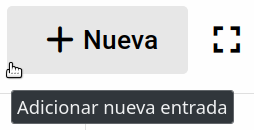
\includegraphics[scale=0.4]{images/prototypes/cdis-create-capture.png}
		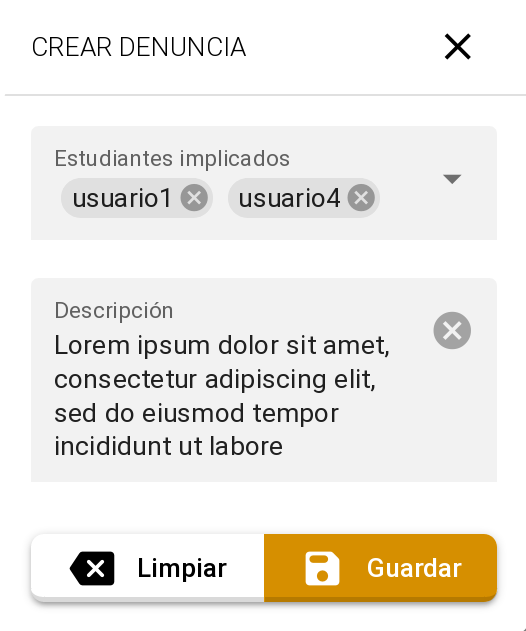
\includegraphics[scale=0.4]{images/prototypes/cdis-create-denuncia-capture.png}}

\end{userstory}
% \begin{userstory}
% 	\storyname{Crear comisi�n disciplinaria}
% 	\storyuser{\authorA}
% 	\storyiter{1}
% 	\storypriority{ Alta }
% 	\storyrisk{ Medio }
% 	\storypoints{1}
% 	\storyprogrammer{\authorA }
% 	\storydescription{El sistema debe permitir registrar una comisi�n disciplinaria. Para ello se le debe brindar al usuario un formulario en el que ingresar los datos de la nueva comisi�n disciplinaria y botones para registrarla en el sistema o cancelar la acci�n.
% 	Los datos a ingresar en el formulario deben ser:
% 		\begin{itemize}
% 		\item Presidente de comisi�n
% 		\item Secretario de comisi�n
% 		\end{itemize}}
% 	\storyobservation{Para registrar una comisi�n tambi�n se necesita la informaci�n de la resoluci�n a la que pertenece, pero, si se permite crear las comisiones en el formulario que se brinda para registrar o modificar una resoluci�n decanal, se debe tomar la resoluci�n a crear o editar como resoluci�n a la que pertenece la comisi�n creada}
% 	\storyinterface{
% 		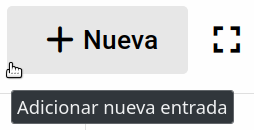
\includegraphics{images/prototypes/cdis-create-capture.png}

% 		}

% \end{userstory}
\begin{userstory}
	\storyname{Crear resoluci�n}
	\storyuser{\authorA}
	\storyiter{1}
	\storypriority{ Alta }
	\storyrisk{ Bajo }
	\storypoints{0.8}
	\storyprogrammer{\authorA}
	\storydescription{El sistema debe permitir registrar una resoluci�n decanal en el sistema. Para ello se le debe brindar al usuario un formulario en el que ingresar los datos de la nueva resoluci�n decanal y botones para registrarla en el sistema o cancelar la acci�n.
		Los datos a ingresar en el formulario deben ser:
		\begin{itemize}
			\item Curso. Puede ser un n�mero correspondiente al a�o o una cCadena de caracteres que lo identifica.
			\item Comisiones disciplinarias
		\end{itemize}}
	\storyobservation{Para registrar una resoluci�n decanal tambi�n se necesita la informaci�n del decano que la emite, para ello se deben tomar los datos del usuario autenticado como decano emisor de la misma.}
	\storyinterface{
		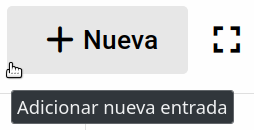
\includegraphics[scale=0.4]{images/prototypes/cdis-create-capture.png}
		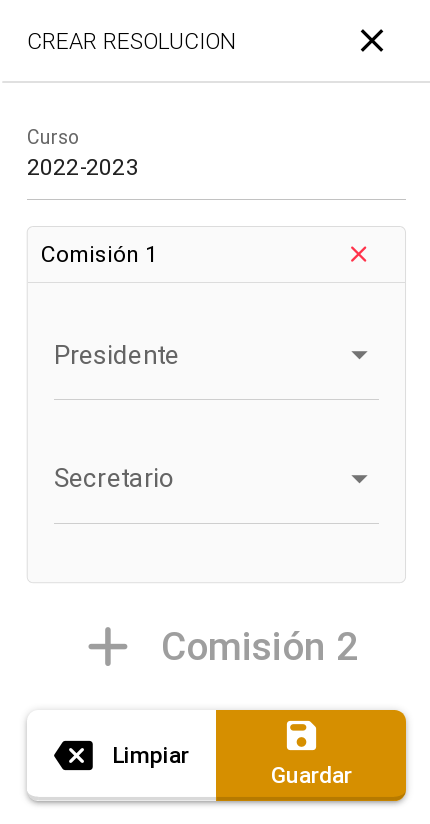
\includegraphics[scale=0.4]{images/prototypes/cdis-create-resolucion-capture.png}}
\end{userstory}
